%----------------------------------------------------------------------------------------
%	PACKAGES AND OTHER DOCUMENT CONFIGURATIONS
%----------------------------------------------------------------------------------------

\documentclass[11pt]{article}

\usepackage[utf8]{inputenc} % Required for inputting international characters
\usepackage[french]{babel}
\usepackage{graphicx} % Import images in document
\graphicspath{ {./images/} }
\usepackage[T1]{fontenc} % Output font encoding for international characters

\usepackage{mathpazo} % Palatino font

\begin{document}

%----------------------------------------------------------------------------------------
%	TITLE PAGE
%----------------------------------------------------------------------------------------

\begin{titlepage} % Suppresses displaying the page number on the title page and the subsequent page counts as page 1
	\newcommand{\HRule}{\rule{\linewidth}{0.5mm}} % Defines a new command for horizontal lines, change thickness here
	
	\center % Centre everything on the page
	
	%------------------------------------------------
	%	Headings
	%------------------------------------------------
	
	\textsc{\LARGE Université de Namur}\\[1.5cm] % Main heading such as the name of your university/college
	
	\textsc{\Large Analyse et modélisation des systèmes de données}\\[0.5cm] % Major heading such as course name
	
	\textsc{\large Travail pratique}\\Groupe 14\\[0.5cm] % Minor heading such as course title
	
	%------------------------------------------------
	%	Title
	%------------------------------------------------
	
	\HRule\\[0.4cm]
	
	{\huge\bfseries Analyse et modélisation du jeu Golden Quest}\\[0.4cm] % Title of your document
	
	\HRule\\[1.5cm]
	
	%------------------------------------------------
	%	Author(s)
	%------------------------------------------------
	
	\begin{minipage}{0.4\textwidth}
		\begin{flushleft}
			\textit{Auteurs}\\
			\large Julien \textsc{Castiaux}
			\\
			\large Kenny \textsc{Warszawski}
		\end{flushleft}

	\end{minipage}
	~
	\begin{minipage}{0.4\textwidth}
		\begin{flushright}
			\large
			\textit{Professeurs}\\
			M. Moussa \textsc{Amrani}\\
			M. Tony \textsc{Leclercq}
		\end{flushright}
	\end{minipage}
	
	% If you don't want a supervisor, uncomment the two lines below and comment the code above
	%{\large\textit{Author}}\\
	%John \textsc{Smith} % Your name
	
	%------------------------------------------------
	%	Date
	%------------------------------------------------
	
	\vfill\vfill\vfill % Position the date 3/4 down the remaining page
	
	{\large\today} % Date, change the \today to a set date if you want to be precise
	
	%------------------------------------------------
	%	Logo
	%------------------------------------------------
	
	%\vfill\vfill
	%
\includegraphics[width=0.2\textwidth]{placeholder.jpg}\\[1cm] % Include a department/university logo - this will require the graphicx package
	 
	%----------------------------------------------------------------------------------------
	
	\vfill % Push the date up 1/4 of the remaining page
	
\end{titlepage}
%----------------------------------------------------------------------------------------
\newpage
%----------------------------------------------------------------------------------------

\section{Plateau de Jeu}

\subsection{Question 1}
Etablir une première version d'un diagramme de classes Uml qui fixe les éléments principaux : le jeu est constitué d'une série de leçons découpées en niveaux.

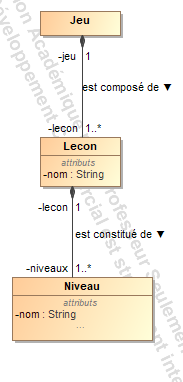
\includegraphics[scale=0.5]{Plateau_5_1.png}

\subsection{Question 2}
Enrichir cette première version avec les détails nécessaires concernant les joueurs et leurs profils, ainsi que les niveaux. 

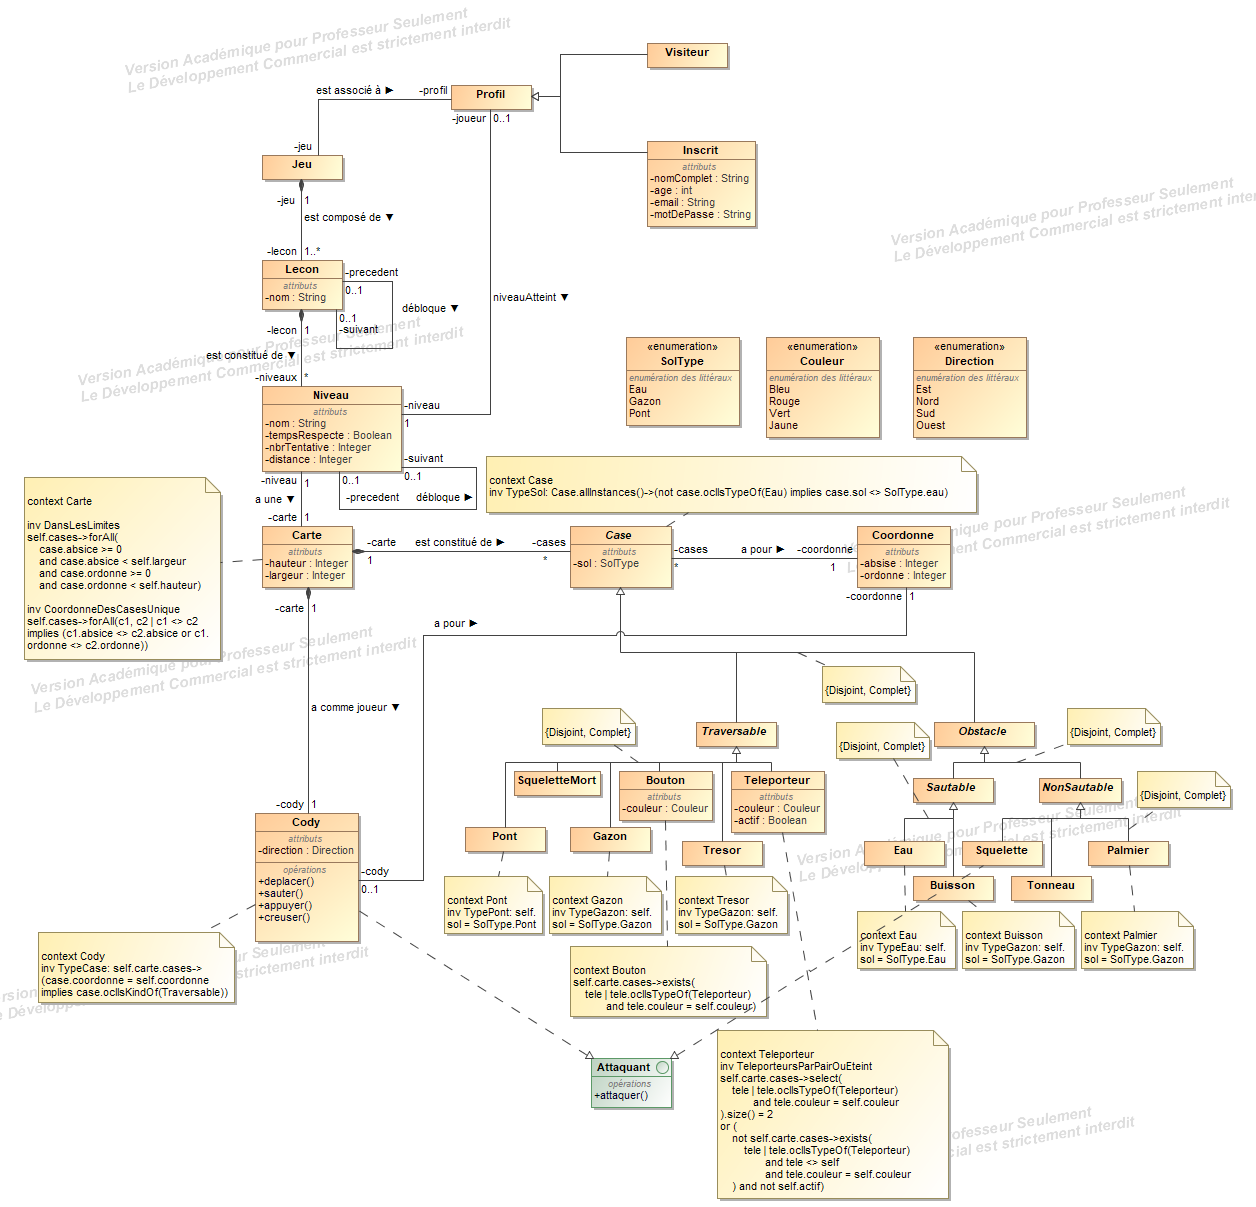
\includegraphics[width=15 cm,height=18 cm]{Plateau_TEX.png}

\subsection{Question 3}
Spécifier les contraintes suivantes, soit à l'aide d'éléments structurels dans le diagramme, éventuellement complétées par des contraintes en Ocl (ceci dépend de la manière dont le diagramme de classes est construit) :

\begin{enumerate}
 
 \item Les coordonnees d'une case ne peuvent excéder les dimensions du niveau
 
 \begin{verbatim}
   context Carte
   inv DansLesLimites
     self.cases->forAll(
       case.coordonne.absice >= 0
       and case.coordonne.absice < self.largeur
       and case.coordonne.ordonne >= 0
       and case.coordonne.ordonne < self.hauteur)
 \end{verbatim}
  
  \item Chaque niveau ne contient qu'un seul Cody, et qu'un seul coffre  
  
  \begin{verbatim}
    
    context Carte
    self.cases->select(
        case | case.oclIsTypeOf(Tresor)
    ).size() = 1    
    
  \end{verbatim}    
  
  En ce qui concerne Cody, la multiplicité répond à cette contrainte.\\
  
  
  \item Un personnage ne peut pas se trouver sur un obstacle 
  
  \item Deux personnages ne peuvent pas partager la même case
  
  \begin{verbatim}
    
   context Cody
   inv TypeCase: self.carte.cases.forAll->(
   case.coordonne = self.coordonne 
      implies case.oclIsKindOf(Traversable)
)    
    
    context Carte
    inv CoordonneDesCasesUnique
    self.cases->forAll(
        c1, c2 | c1 <> c2 
        implies (c1.absice <> c2.absice 
                 or c1.ordonne <> c2.ordonne))    
    
  \end{verbatim}     
  
  Nous considérons que les squelettes sont des cases de type Obstacle. Il est donc impossible qu'un squelette se trouve sur un obstacle du fait de l'unicité des cases reprise par la contrainte OCL ci-dessus. Cody doit être sur une case Traversable et donc ne peut pas être sur un squelette.\\
  
  \item Le coffre doit se trouver sur du gazon
  
  \begin{verbatim}
    context Tresor
    inv TypeGazon: self.sol = SolType.Gazon
  \end{verbatim}     
  
  \item  Un niveau doit toujours comporter deux tunnels de teleportation de même couleur, ou le tunnel unique doit être initialement fermé 
  
  \begin{verbatim}
    context Teleporteur
    inv TeleporteursParPairOuEteint
    self.carte.cases->select(
           tele | tele.oclIsTypeOf(Teleporteur)
             and tele.couleur = self.couleur).size() = 2
         or (
           not self.carte.cases->exists(
               tele | tele.oclIsTypeOf(Teleporteur)
                 and tele <> self
                 and tele.couleur = self.couleur
    ) and not self.actif)
  \end{verbatim}     
  
  \item Un levier de téléportation ne peut être présent que s'il existe des tunnels de la même couleur
  
  \begin{verbatim}
    context Bouton
    self.carte.cases->exists(
       tele | tele.oclIsTypeOf(Teleporteur)
           and tele.couleur = self.couleur)
  \end{verbatim}     
  
  \item Un palmier ou un buisson doivent obligatoirement être posé sur du gazon (sinon, il ne peut pas pousser).
  
  \begin{verbatim}
    context Buisson
    inv TypeGazon: self.sol = SolType.Gazon
    
    context Palmier
    inv TypeGazon: self.sol = SolType.Gazon
  \end{verbatim}     
  
\end{enumerate}

\section{Langage Play}

\subsection{Question 5}

Etablir une première version d'un diagramme de classe Uml qui fixe les éléments principaux :un Program(me) Play est un ensemble de procédures (dont l'une est la procédure principale).

 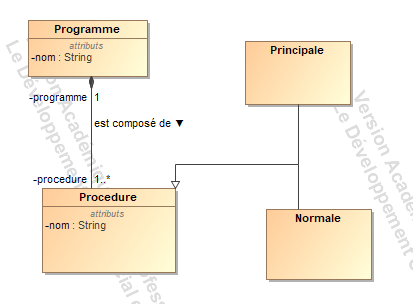
\includegraphics[scale=0.5]{Play_Q1.png}

\subsection{Question 6}

Modéliser le concept de procédure à partir d'une classe Procedure.

 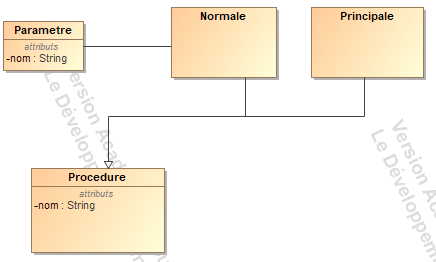
\includegraphics[scale=0.5]{Play_Procedure.png}

\subsection{Question 7}

Modéliser le concept d'expression comme indiqué en Section 3.3, à partir d'une classe Expression.

 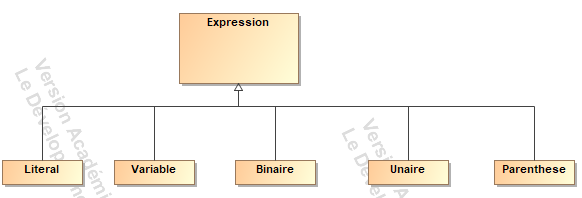
\includegraphics[scale=0.5]{Play_Expression.png}


\end{document}
